\documentclass{scalatekids-article}
\usepackage[official]{eurosym}
\usepackage[english]{babel}
\usepackage[bottom]{footmisc}
\begin{document}
\pagestyle{fancy}
\fancyhf{}
\lhead{
  
\includegraphics[height=1cm, width=1cm, keepaspectratio=true]{ablogoSmall.png} \emph{Actorbase - ScalateKids}}
\rhead{
  \slshape \leftmark
}
\setlength{\headsep}{1.2cm}
% pagestyle set to 'n di m'
\rfoot{\thepage\hspace{1pt}of \pageref{LastPage}}
\lfoot{User Manual 2.0.0}
\newgeometry{top=3.5cm}
\begin{titlepage}
  \begin{center}
    \begin{center}
      
\includegraphics[width=10cm]{ablogo.png}
    \end{center}
    \vspace{1cm}
    \begin{Huge}
      \begin{center}
        \textbf{User Manual}
      \end{center}
    \end{Huge}
    \vspace{11pt}
    \bgroup
    \def\arraystretch{1.3}
    \begin{tabular}{r|l}
      \multicolumn{2}{c}{\textbf{Document Information}} \\
      \hline
      \setbox0=\hbox{0.0.1\unskip}\ifdim\wd0=0pt
      \\
      \else
      \textbf{Version} & 2.0.0\\
      \fi
      \textbf{Editing} & \multiLineCell[t]{Alberto De Agostini}\\
      \textbf{Verification} & \multiLineCell[t]{Michael Munaro}\\
      \textbf{Approvation} & \multiLineCell[t]{Davide Trevisan}\\
      \textbf{Use} & External\\
      \textbf{Distribution list} & \multiLineCell[t]{ScalateKids\\Prof. Tullio Vardanega\\Prof. Riccardo Cardin}\\
    \end{tabular}
    \egroup
    \vspace{22pt}
  \end{center}
\end{titlepage}
\restoregeometry
\clearpage
\pagenumbering{Roman}
\setcounter{page}{1}
\begin{flushleft}
  \vspace{0cm}
  {\large\bfseries History log}
\end{flushleft}
\vspace{0cm}
\begin{center}
  \begin{longtable}{| l | l | l | l | p{5cm} |}
    \hline
    2.0.0 & Davide Trevisan & Project Manager & 2016-06-15 & Document Approved\\
    \hline
    1.2.0 & Michael Munaro & Verifier & 2016-07-02 & Verified changes on section 2\\
    \hline
    1.1.1 & Alberto De Agostini & Programmer & 2016-07-01 & Modified section 2 to reflect changes on CLI\\
    \hline
    1.1.0 & Michael Munaro & Verifier & 2016-06-30 & Verified glossary\\
    \hline
    1.0.1 & Alberto De Agostini & Programmer & 2016-05-30 & Added glossary\\
    \hline
    Version & Author & Role & Date & Description \\
    \hline
    1.0.0 & Michael Munaro & Project Manager & 2016-05-09 & Document approved\\
    \hline
    0.1.0 & Marco Boseggia & Verifier & 2016-05-07 & Verified CLI section\\
    \hline
    0.0.2 & Alberto De Agostini & Programmer & 2016-05-04 & Added CLI section\\
    \hline
    0.0.1 & Alberto De Agostini & Programmer & 2016-05-04 & Created document structure\\
    \hline
  \end{longtable}
\end{center}
\tableofcontents
\newpage
\pagenumbering{arabic}
\section{Summary}

\subsection{Document purpose}
This document represents the user manual for the \textit{actorbase} application
and describes in detail every single feature of it. Actorbase is a database that
comes with two different software modules capable of interacting with it; the
user can use both these modules, so this document will present them in two
different sections.

\subsection{Product purpose}

The purpose of the project is the realization of a key-value type
\gloss{NoSQL} database,
massively concurrent and oriented to the management of heavy load of data by
using the \gloss{actor} model.

\subsection{Glossary}
Every technical word, some words that can be misunderstood and all of acronyms are defined in the glossary in the appendix \ref{sec:Glossary}.
Every word that is in the glossary will be marked with a subscript ”G”.

% \subsection{References}

% \subsubsection{Normative} % TODO check, translated with wordreference

% \subsubsection{Informational} % TODO check, translated with wordreference

% TODO parte server: installazione, configurazione, accensione, spegnimento

% TODO mettere una sezione in cui si spiega cosa è una collection, un item, tutto quel che bisogna descrivere

%%%%%%%%%%%%%%%%%%%%%%%%%%%%%%%%%%%%%%%%%%%%%%%%%%%%%%%%%%%%%%%%%%%%
%%%                          CLI part                            %%%
%%%%%%%%%%%%%%%%%%%%%%%%%%%%%%%%%%%%%%%%%%%%%%%%%%%%%%%%%%%%%%%%%%%%
\section{Actorbase by Command Line Interface}

\subsection{DSL}

The DSL (Domain System Language), upon which the \textit{actorbase} CLI (Command
Line Interface) is based, has been developed trying to make it as close as possible
to spoken English in order to make it easier to understand.

\subsection{Error management}

There are two kinds of errors that are shared by every command which will be
now explained:
\begin{itemize}
\item In case of an unrecognized command, or in case of a typographical error,
  the CLI will show an unrecognized command error followed by a list of all
  the commands available to the user;
\item In case of a connection error, which can be caused by not receiving a
  response from the server in a predetermined time, the CLI will show a
  timeout connection error.
\end{itemize}
There are some errors that are specific to some commands, these will be explained
in the section dedicated to the commands that cause them.

% TODO scrivere anche i tipi di dato possibili da inserire? tipo le stringhe devono essere in " ", permission su addcontributor può essere vuoto, r o rw ecc

\subsection{Password requirements}
\label{sec:passwordrequirement}
Every password must contain at least one uppercase, one lowercase letter and one
digit and be at least 8 characters long.\\
The default password of actorbase for users that are just added or after a password reset is \texttt{Actorb4se}.

\subsection{Running and configurating the actorbase CLI} % TODO da fare
To run the Actorbase CLI some requirements needs to be fullfilled before starting it.\\
The user has to download and install all the software requirements (see link) and an instance of 
actorbase server must be running.\\
When all those requirements are fullfilled to start the CLI the use has to open a terminal and type:\\
\begin{center}
  \texttt{java -jar <pathToActorbaseCLIJar> -u <username> -h <host> -p <port>}
\end{center}
Where the username is the username with which you want to login in actorbase, host is the ip where 
actorbase is listening for requests and the port is the port where actorbase is listening for 
requests.\\All those parameters can be omitted, if omitted the CLI will try to connect with the 
default user ``anonymous'' in the default host ``localhost'' with default port ``9999''. 

\subsection{Operations on collections not of your own}
\label{sec:contributoroperations}
If the user is a contributor to a collection the syntax to make every operations that involves selecting one or more 
\gloss{collections} is a little different. When the user has to insert the name of a \gloss{collection} instead of 
just typing \texttt{``<collection name>''} the user has to insert \texttt{``<collection owner username>.<collection name>''}.\\This way the user tells actorbase to operate on a collection not of his own.\\This is also to let the user to 
create a \gloss{collection} with the same name of a \gloss{collection} of which he has access to but it is not of 
his own. 

\subsection{Operations}

The following sections requires the actorbase CLI to be configured and
running (see \hyperref[sec:configurationcli]{Configure CLI}).\\
The features described are divided by the type of the user.\\

\subsubsection{Acceptable values}
Every operations that accepts parameters like the collection name or the key of 
an item has some limitations on the value:
\begin{itemize}
  \item Keys and collection names must contains only alphanumeric characters.
\end{itemize}


\subsubsection{Standard user operations}
\label{sec:everyuser}

\paragraph{Exit from CLI}
\textbf{Description:} every user can exit from the actorbase CLI
using this procedure.\\
\textbf{How to:} type \texttt{exit} on the CLI

%\subsubsection{Unauthenticated user}
%\label{sec:unauthenticateduser}

\paragraph{Help - generic help}
\label{sec:generichelp}
\textbf{Description:} this feature allows the user to ask for help.\\
The CLI will answer with a list of all the possible operations alongside
their right syntax.\\
%The list of functionalities differs with the user type (e.g. authenticated user has more features than an unauthenticated one).\\
\textbf{How to:}
\begin{itemize}
\item Type \texttt{help}
\item The CLI will display a help message
\end{itemize}

%\subsubsection{Authenticated user}
%\label{sec:authenticateduser}

%\paragraph{Help - generic help}

%See \hyperref[sec:generichelp]{Generic help}

\paragraph{Help - specific help}
\label{sec:specifichelp}
\textbf{Description:} this feature allows the user to ask for help for
a specific command.\\
The CLI will answer with a message explaining how to use that command and
which parameters it needs.\\
\textbf{How to:}
\begin{itemize}
\item Type \texttt{help <command name>}
\item The CLI will display a message explaining how to use the command and his syntax
\end{itemize}
\textbf{Possible errors:} the CLI will answer with self explanatory error messages
\begin{itemize}
\item If the command name the user typed is not a command of the actorbase CLI
\end{itemize}

\paragraph{Create a collection}
\label{sec:createcollection}
\textbf{Description:} this feature allows the user to create a
\gloss{collection} into the database.\\
\textbf{How to:}
\begin{itemize}
\item Type \texttt{createCollection ``<collection name>''}
\item The CLI will display a message explaining how to use the command and what parameters it needs
\end{itemize}
\textbf{Possible errors:} the CLI will answer with self explanatory error messages
\begin{itemize}
\item If the \gloss{collection} the user wants to create is already in the server the CLI will answer with a message
\end{itemize}

\paragraph{List collections}
\label{sec:listcollection}
\textbf{Description:} this feature allows the user to see a list of
the \gloss{collections} he has permission on.\\
\textbf{How to:}
\begin{itemize}
\item Type \texttt{listCollection}
\item The CLI will display a list of all the \gloss{collections} the user has
  permission on
\end{itemize}

\paragraph{Delete a collection}
\label{sec:deletecollection}
\textbf{Description:} this feature allows the user to remove a \gloss{collection} and all the items inside it from the database.\\
\textbf{How to:}
\begin{itemize}
\item Type \texttt{deleteCollection ``<collection name>''}
\end{itemize}

\paragraph{Add a contributor to a collection}
\label{sec:addcontributor}
\textbf{Description:} this feature allows the user to add a contributor
to a \gloss{collection} of his own. The contributor will have the permission to operate on the selected \gloss{collection} depending on the what permissions the user decide to give him.\\
\textbf{How to:}
\begin{itemize}
\item Type \texttt{addContributor ``<username>'' to ``<collection name>'' <ReadOnly|ReadWrite>}
\end{itemize}
\textbf{Possible errors:} the CLI will answer with self explanatory error messages
\begin{itemize}
\item If the \gloss{collection} the user wants to add the contributor to does not exists on the server or it is not a \gloss{collection} the user own
\item If the username the user typed does not correspond with a user registered in actorbase
\item If the permissions the user typed are not ReadOnly or ReadWrite
\end{itemize}

\paragraph{Remove contributor from a collection}
\label{sec:removecontributor}
\textbf{Description:} this feature allows the user to remove a contributor from a \gloss{collection} of his own.\\
\textbf{How to:}
\begin{itemize}
\item Type \texttt{removeContributor ``<username>'' from ``<collection name>''}
\end{itemize}
\textbf{Possible errors:} the CLI will answer with self explanatory error messages
\begin{itemize}
\item If the \gloss{collection} the user wants to remove the contributor from does not exists on the server or it is not a \gloss{collection} the user owns
\item If the username the user typed does not correspond with a user registered in actorbase
\end{itemize}

\paragraph{Export one or more collections to file}
\label{sec:export}
\textbf{Description:} this feature allows the user to export one or more \gloss{collections} he has access to.\\
The filename the user insert can be a relative or absolute path; if the path is not present, it will be created.\\
%todo davvero?
The \gloss{collection} list can contain zero or more \gloss{collections}' name, if empty it will export 
all the \gloss{collections} the user has access to (possibly resulting in an expensive operation).\\
To export collections that you are contributor on see \hyperref[sec:contributoroperations]{contributor operations}.\\
\textbf{How to:}
\begin{itemize}
\item Type \texttt{export ``<collection name1>'', ``<collection name2>'', ... , to ``<filename>''}
\end{itemize}
\textbf{Possible errors:} the CLI will answer with self explanatory error messages
\begin{itemize}
\item If at least one of the \gloss{collections}' name the user inserted does not exist on the server
\item If the filename the user inserted contains a path that is not valid
\end{itemize}

The produced JSON file follow some rules explained in \hyperref[sec:JSONFormat]{JSON format}.

\paragraph{Insert item}
\label{sec:insertitem}
\textbf{Description:} this feature allows the user to insert an item in a particular \gloss{collection}.\\
With this command it's not possible to overwrite an item, to do that see \hyperref[sec:updateditem]{Update item}.\\
The <key> is a String representing the key of the item the user wants to insert.\\
The <value> can be anything the user wants to insert and it represent the value of the item itself.\\
If the user wants to insert the item in a non existing \gloss{collection} the server
will automatically create that \gloss{collection}.\\
To insert in a collection that you are contributor on see \hyperref[sec:contributoroperations]{contributor operations}.\\
\textbf{How to:}
\begin{itemize}
\item Type \texttt{insert ( ``<key>'' -> ``<value>'' ) to ``<collection name>''}
\end{itemize}
\textbf{Possible errors:} the CLI will answer with self explanatory error messages
\begin{itemize}
\item If the \gloss{collection} the user wants to insert the item in a \gloss{collection} in which he is a contributor with no write premissions
\item If the user decides to insert an item with an already existing key in that \gloss{collection} and the overwrite option has not been chosen.
\end{itemize}

\paragraph{Update item}
\label{sec:updateitem}
\textbf{Description:} this feature allows the user to insert an item in a particular \gloss{collection}.\\
With this command it's possible to overwrite an item already existing.\\
The <key> is a String representing the key of the item the user wants to insert.\\
The <value> can be anything the user wants to insert and it represent the value of the item itself.\\
If the user wants to insert the item in a non existing \gloss{collection} the server
will automatically create that \gloss{collection}.\\
To insert in a collections that you are contributor on see \hyperref[sec:contributoroperations]{contributor operations}.\\
\textbf{How to:}
\begin{itemize}
\item Type \texttt{update ( ``<key>'' -> ``<value>'' ) to ``<collection name>''}
\end{itemize}
\textbf{Possible errors:} the CLI will answer with self explanatory error messages
\begin{itemize}
\item If the \gloss{collection} the user wants to insert the item in a \gloss{collection} in which he is a contributor with no write premissions
\end{itemize}

\paragraph{Import from file}
\label{sec:import}
\textbf{Description:} this feature allows the user to insert a list of \gloss{collections} and items from a file.\\
The file has to be formatted as specified in (see \hyperref[sec:JSONFormat]{JSON format})\\
\textbf{How to:}
\begin{itemize}
\item Type \texttt{import ``<path/to/filename>''}
\end{itemize}
\textbf{Possible errors:} the CLI will answer with self explanatory error messages
\begin{itemize}
\item If the file is not a JSON file
\item If the file is not formatted as specified in \hyperref[sec:JSONFormat]{JSON format}
\item If the file specified the creation of \gloss{collection} that the user can not create (see \hyperref[sec:createcollection]{create collection})
\item If the file specified the insertion of items that the user can not insert
\end{itemize}

\paragraph{Remove item}
\label{sec:removeitem}
\textbf{Description:} this feature allows the user to remove an item from a \gloss{collection}.\\
<key> represents the key of the item the user wants to remove from the \gloss{collection}.\\
To remove items from collections that you are contributor on see \hyperref[sec:contributoroperations]{contributor operations}.\\
\textbf{How to:}
\begin{itemize}
\item Type \texttt{remove ``<key>'' from ``<collection name>''}
\end{itemize}
\textbf{Possible errors:} the CLI will answer with self explanatory error messages
\begin{itemize}
\item If the \gloss{collection} the user typed does not exist in the server or if the user does not have permission to remove items from
\end{itemize}

\paragraph{Find item}
\label{sec:find}
\textbf{Description:} this feature allows the user to search for particular items in the database. There are different types of search based on the parameters typed.\\
To search from collections that you are contributor on see \hyperref[sec:contributoroperations]{contributor operations}.\\

\subparagraph{Search items in one or more collections}
\textbf{Description:} this feature lets the user search for an item in one or more \gloss{collections}; 
the user must have the permission to read these \gloss{collections}.\\
\textbf{How to:}
\begin{itemize}
\item Type \texttt{find ``<key>'' from ``<collection name 1>'', ``<collection name 2>'', ... , ``<collection name N>''}
\end{itemize}
\textbf{Possible errors:} the CLI will answer with self explanatory error messages
\begin{itemize}
\item If at least one of the \gloss{collections} does not exist on the server or if the user has not read permission on some of the \gloss{collections}
\end{itemize}

\subparagraph{Search items in the entire database}
\textbf{Description:} this feature lets the user search for an item in the entire database visible to him.\\
\textbf{How to:}
\begin{itemize}
\item Type \texttt{find ``<key>''}
\end{itemize}

\subparagraph{Search for all the items of one or more collections}
\textbf{Description:} this feature lets the user retrieve all the items contained in one or more \gloss{collections}.\\
\textbf{How to:}
\begin{itemize}
\item Type \texttt{find from ``<collection name 1>'', ``<collection name 2>'', ... , ``<collection name N>''}
\end{itemize}
\textbf{Possible errors:} the CLI will answer with self explanatory error messages
\begin{itemize}
\item If at least one of the \gloss{collection} does not exist on the server or if the user doesn't have access to it
\end{itemize}

\subparagraph{Get all database items grouped by collection}
\textbf{Description:} this feature lets the user to retrieve all the items contained in the section of the database that is visible to him grouped by \gloss{collection}.\\
This operation could be expensive.\\
\textbf{How to:}
\begin{itemize}
\item Type \texttt{find}
\end{itemize}

\paragraph{Change password}
\label{sec:changepassword}
\textbf{Description:} this feature allows the user to change his password.\\
\textbf{How to:}
\begin{itemize}
\item Type \texttt{changePassword}
\item Type \texttt{``<old password>''}
\item Type \texttt{``<new password>''}
\item Type \texttt{``<repeat new password>''}
\end{itemize}
\textbf{Possible errors:} the CLI will answer with self explanatory error messages
\begin{itemize}
\item If the old password typed was wrong
\item If the new password typed doesn't follow the rules explained \hyperref[sec:passwordrequirement]{here}
\item If the repeated new password is no the same as the new password typed before.
\end{itemize}

\subsubsection{Administrator user operations}
\label{sec:administratoruser}

\paragraph{Add user}
\label{sec:adduser}
\textbf{Description:} this feature allows the administrator to add a new user to the database with a default password (see \hyperref[sec:passwordrequirement]{password section}).\\
\textbf{How to:}
\begin{itemize}
\item Type \texttt{addUser ``<username>''}
\end{itemize}

\paragraph{Remove user}
\label{sec:removeuser}
\textbf{Description:} this feature allows the administrator to remove an user from the database.\\
\textbf{How to:}
\begin{itemize}
\item Type \texttt{removeUser ``<username>''}
\end{itemize}

\paragraph{Reset password}
\label{sec:resetpassword}
\textbf{Description:} this feature allows the administrator to change the password of an user to the one that was set by default (see \hyperref[sec:passwordrequirement]{password section}).\\
\textbf{How to:}
\begin{itemize}
\item Type \texttt{resetPassword ``<username>''}
\end{itemize}

\paragraph{List users}
\label{sec:listusers}
\textbf{Description:} this feature allows the administrator to get a list of all the users 
registrated in actorbase.\\
\textbf{How to:}
\begin{itemize}
\item Type \texttt{listUsers}
\end{itemize}

\newpage
\appendix

\section{JSON file format for import}
\label{sec:JSONFormat}
Exporting data from \textbf{Actorbase} generate a well-formatted JSON file, and the same format must be
used for import data to filesystem, e.g.:

\begin{figure}[H]
  \begin{center}
    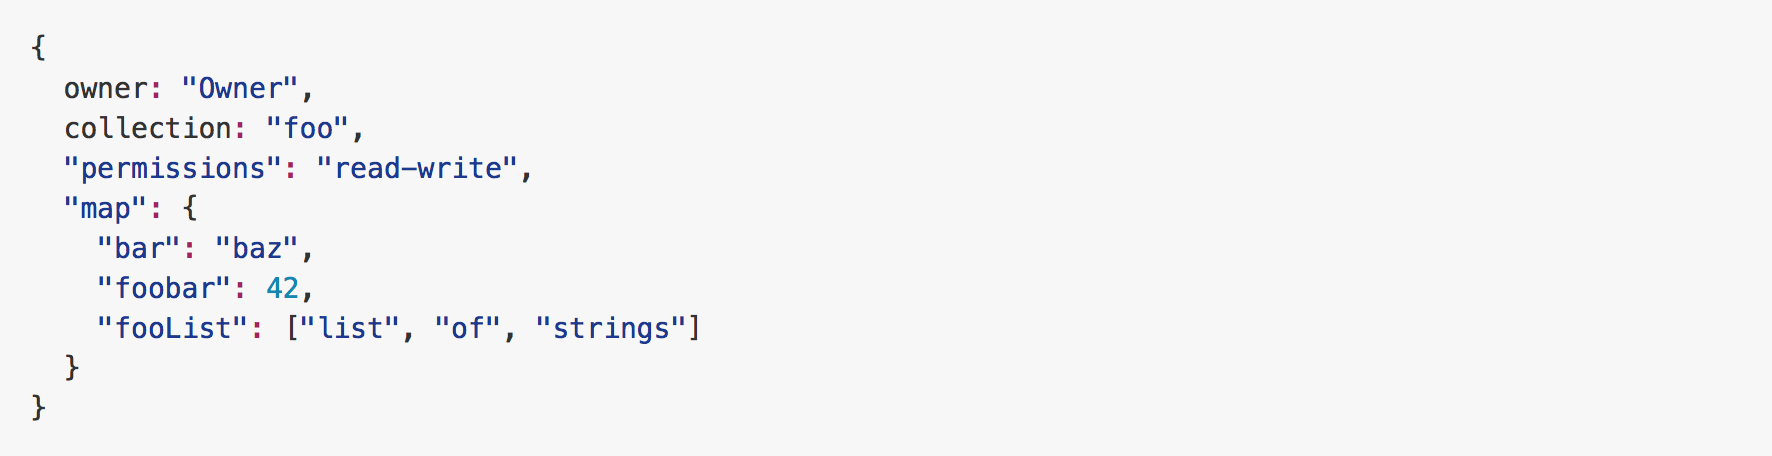
\includegraphics[width=0.5\textwidth,keepaspectratio]{RQ/JSONformat.png}
    \caption{JSON well-formatted file}
  \end{center}
\end{figure}

\listoffigures

\section{Glossary}
\label{sec:glossary}
\subsection{A}
  \glossDef{Actor} A computational entity that, in response to a message
  it receives, can send messages to other actors, create new ones, change its
  behaviour for the next message incoming\label{actor} \\
\subsection{C}
  \glossDef{Collection} A data-structure constituted by a list of key-value items\label{coll} \\
\subsection{N}
  \glossDef{NoSql} A NoSQL database provides a mechanism for storage and retrieval
  of data which is modeled in means other than the tabular relations used in
  relational databases. Key-value (KV) stores use the associative array (also known
  as a map or dictionary) as their fundamental data model.\label{nosql}


\end{document}